\documentclass[12pt,letterpaper]{article}

\usepackage{natbib}

\usepackage[T1]{fontenc}

\usepackage{tabulary}
\usepackage{float}
\restylefloat{table}

\usepackage{ucs}

\usepackage[utf8x]{inputenc}

\usepackage[spanish]{babel}
\spanishdecimal{.}

\usepackage{graphicx}
\graphicspath {{Images/}} % Relative path to tex file

\newcommand{\iee}{\emph{i.e.} }
\newcommand{\egg}{\emph{e.g.} }

\newcommand{\mc}[3]{\multicolumn{#1}{#2}{#3}}

\newcommand{\bfs}[1]{{\bfseries\small #1}}

\newlength{\spacing}
\setlength{\spacing}{\baselineskip}

\newcommand{\X}{$\times$}
\newcommand{\nspace}[1]{\setlength{\baselineskip}{#1\spacing}}
\newenvironment{linespacing}[1]{\nspace{#1}}{}

\title{Protocolo de Tesis}
\author{}
\date{18 de Agosto de 2016}

\begin{document}

\maketitle

\bibliographystyle{apalikesp}

\begin{linespacing}{1.5}

\section{Datos generales}
\begin{table}[htb]
\centering
\begin{tabular}{|c|l|}\hline
Título: &
\mc {1} {|p{0.78\textwidth}|} {\textbf{Estimación de la pose de un \textit{UAV} basado en mediciones de un sistema de video monocular.}} \\\hline              
Autor: & \textbf{Rodrigo Cuevas Centeno} \\\hline
Posgrado: & \textbf{Maestría en Ciencias de la Computación}\\\hline
Asesores: & \textbf{Dr. Arturo Espinosa Romero, Dr. Ricardo Legarda Sáenz} \\\hline
\end{tabular}
\end{table}

\section{Introducción}

Los vehículos aéreos no tripulados (Unmanned aerial vehicles ó \textit{UAVs}) juegan un papel importante en la recolección de información y la fusión de datos. Debido a su movilidad y a la complejidad de los ambientes en los que son desplegados, un conocimiento constante de su posición así como la capacidad para evitar colisiones es esencial. \\Los \textit{UAVs} pueden causar peligro si su señal de \textit{GPS} no se encuentra disponible o es débil, por eso un sistema capaz de estimar su posición basada solo en las imágenes de una cámara puede ofrecer una solución ante dicha problemática.

\subsection{Antecedentes}

\cite{Maldonado_Thesis} en su tesis de maestría realizó la estimación de la pose de un \textit{UAV} usando mosaicos de imágenes, además de construir un dispositivo que tiene la tarea de grabar y realizar los cálculos requeridos y usando un papalote para hacer volar dicho dispositivo; Esta tesis es una continuación de dicho trabajo con la diferencia de que se pretende no depender tanto del \textit{GPS} y la \textit{IMU}, así como también probar nuevas implementaciones para mejorar la precisión de la estimación.

\section{Objetivo de la tesis}

Estimar la pose de un vehículo aéreo no tripulado basándose en información obtenida a partir de imágenes en tiempo real de un sistema de video monocular abordo, así como de los sensores inerciales incluidos.

\subsection{Objetivos Particulares}

\begin{itemize}
\item Utilizar un modelo del sistema que describa la pose en términos de las variables de instrumentación.
\item Implementar un método que permita la selección adecuada de las características (\textit{features}) del paisaje observado considerando que no se tiene ningún punto de referencia previo.
\item Proponer un método que permita el seguimiento cuadro por cuadro de las características encontradas (\textit{tracking}) considerando que debe tener cierta robustez ante las imágenes borrosas obtenidas dado el movimiento del \textit{UAV}.
\item Proponer e implementar un método que permita la estimación de la pose (seis grados de libertad) de un objeto minimizando el error propio del método.
\end{itemize}

\section{Marco teórico}

Los tres elementos principales requeridos para la estimación de la pose de un \textit{UAV} son:

\begin{itemize}
\item Obtención de características.
\item Seguimiento.
\item Cálculo de la pose.
\end{itemize}

En el campo de visión computacional y procesamientos de imágenes, una \textbf{característica} es un pedazo de información relevante para resolver alguna tarea computacional relacionada a cierta aplicación. Uno de los pasos mas importantes al tratar de resolver la estimación de pose de un \textit{UAV} es la detección de las características en una imagen. El seguimiento (\textit{tracking}) es el proceso de localizar un objeto en movimiento a través del tiempo usando una cámara y se utiliza para establecer el movimiento que realizo una característica durante el recorrido del \textit{UAV}. \\
\cite{3DPose} realiza seguimiento calculando las homografías (relación entre dos imágenes en la misma superficie planar de un espacio) entre cada cuadro de una imagen de video, eliminando a los puntos atípicos con ayuda del algoritmo \textit{RANSAC}, esto ayuda en la implementación de algoritmo llamado \textit{Pyramidal Lucas–Kanade}, el cual es una de los múltiples algoritmos que existen para realizar seguimiento de características y uno de los cuales con el que se realizaran pruebas dada su eficiencia de cálculo según la literatura. \\
En visión computacional y la robótica, una tarea particular es la de identificar objetos específicos en una imagen, y determinar la posición y orientación relativa del objeto en algún sistema de coordenadas. A la combinación de posición y orientación es llamada \textbf{pose}. \cite{UKF} usan el algoritmo llamado \textit{Unscented Kalman Filter} para realizar la estimación de la pose de un \textit{UAV} y es uno de los algoritmos que han demostrado buenos resultados ala hora de realizar estimaciones.

\section{Metodología}

La fase de experimentación que se realizara durante la tesis para la validación del modelo de estimación y el calculo de la pose es el siguiente:\\
Se tiene una cámara en un plano aéreo (montada en un \textit{UAV}) la cual está en movimiento constante en alguna dirección, se encuentra posicionada mirando hacia abajo y estará tomando video continuamente mientras realiza su desplazamiento en el aire. \\
Las imágenes obtenidas serán procesadas en un sistema de cómputo que se encontrará conectado a la cámara, es decir, dicho sistema estará localizado en el aire.
El sistema de cómputo al procesar las imágenes seleccionara las mejores características que sirvan como puntos de referencia.
Basándose en los puntos de referencia encontrados en cada imagen del vídeo se calcula la homografía.
Con las homografías obtenidas por cada imagen se pueden aplicar métodos para encontrar la pose actual del \textit{UAV}.\\
La parte de experimentación se realizara en dos fases:

\begin{enumerate}
\item En la primera fase las pruebas serán realizadas sobre una retícula en un ambiente controlado en el laboratorio usando solo la cámara y simulando algunas situaciones reales para revisar que los métodos implementados estén desempeñando su objetivo de manera adecuada.
\item Durante la segunda fase, después de verificar el correcto funcionamiento y robustez en un ambiente de controlado, se implementaran los métodos en un \textit{UAV} en un ambiente natural.
\end{enumerate}

\begin{figure}[H]
\centering
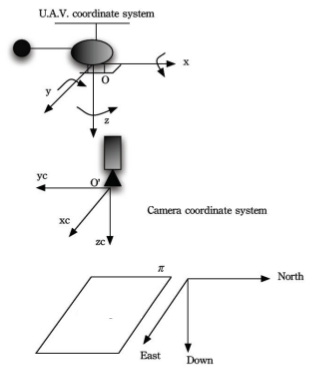
\includegraphics[width=.55\linewidth]{metodologia.png}
\caption{Esquema general. \cite{Martinez2011}.}
\end{figure}

\section{Recursos}
El siguiente material es necesario para llevar a cabo ésta tesis:

\begin{itemize}
\item Cámara digital.
\item Vehículo aéreo no tripulado con \textit{GPS}, \textit{IMU} y \textit{GPU}.
\item Retícula.
\item Computadora personal con \textit{GPU}.
\end{itemize}

\section{Calendario de actividades}

\begin{enumerate}
\item Revisión de la literatura sobre selección de características, seguimiento y estimación de pose de un \textit{UAV}.
\item Evaluación de técnicas de selección de características e implementación.
\item Evaluación de métodos de seguimiento con el fin de elegir el mas eficiente y su implementación.
\item Evaluación de métodos de estimación de pose e implementación de algún de estos métodos adaptándolo al problema definido.
\item Experimentación en un ambiente controlado en laboratorio,
\item Experimentación en un ambiente natural.
\item Ajustes a los métodos basado en resultados del ambiente natural y una fase de experimentación adicional.
\item Documentación de la tesis.
\end{enumerate}

\begin{table}[H]
\centering
\footnotesize
\begin{tabulary}{1.2\textwidth}{|L|C|C|C|C|C|C|C|C|C|C|C|C|C|C|}
\hline
\multicolumn{1}{|c|}{Actividades} & Jun & Jul & Ago & Sep & Oct & Nov & Dic & Ene & Feb & Mar & Abr & May & Jun & Jul \\ \hline
1. Lit.                          & x   & x   & x   &     &     &     &     &     &     &     &     &     &     &     \\ \hline
2. Eva. Car.                     &     & x   & x   & x   &     &     &     &     &     &     &     &     &     &     \\ \hline
3. Eva. Seg.                     &     &     & x   & x   & x   & x   &     &     &     &     &     &     &     &     \\ \hline
4. Eva. Pose.                    &     &     &     &     &     & x   & x   & x   & x   &     &     &     &     &     \\ \hline
5. Exp. Lab.                     &     & x   & x   & x   & x   & x   & x   &     &     &     &     &     &     &     \\ \hline
6. Exp. Amb.                     &     &     &     &     &     & x   & x   & x   & x   &     &     &     &     &     \\ \hline
7. Aju.                          &     &     &     &     &     &     &     & x   & x   & x   & x   & x   &     &     \\ \hline
8. Doc                           & x   & x   & x   & x   & x   & x   & x   & x   & x   & x   & x   & x   & x   & x   \\ \hline
\end{tabulary}
\caption{Cronograma de actividades.}
\end{table}

\end{linespacing}

\begin{linespacing}{1.0}
\addcontentsline{toc}{section}{Referencias}
\bibliography{References}
\end{linespacing}

\end{document}
